\documentclass{exam}
\usepackage{amssymb}
\usepackage{lipsum} 
\usepackage{graphicx}
\usepackage[
backend=biber
]{biblatex}
\addbibresource{refs.bib}

\newcommand\labnr{5}
\newcommand\lab{Lab \labnr\ - Graph Representations, Depth First Search, Breadth First Search}

\newcommand\uni{Technical University of Cluj-Napoca}
\newcommand\course{Data Structures \& Algorithms}

\newcommand\lvlez{$\bigstar$}
\newcommand\lvlmed{\lvlez\lvlez}
\newcommand\lvlhard{\lvlmed\lvlez}
\newcommand\lvlvhard{\lvlhard\lvlez}


\pagestyle{headandfoot}
\firstpageheader{}{}{}
\firstpagefootrule
\firstpageheadrule
\firstpagefooter{\sc\uni}{}{\sc\course, Lab \labnr}
\runningheader{\sc\uni}{}{\sc\course, Lab \labnr}
\runningheadrule
\runningfootrule
\runningfooter{}{\thepage}{}

\usepackage{listings}
\usepackage{xcolor}
\usepackage{svg}

\definecolor{codegreen}{rgb}{0,0.6,0}
\definecolor{codegray}{rgb}{0.5,0.5,0.5}
\definecolor{codepurple}{rgb}{0.58,0,0.82}
\definecolor{backcolour}{rgb}{0.95,0.95,0.92}

\lstdefinestyle{mystyle}{
    commentstyle=\color{codegreen},
    keywordstyle=\color{magenta},
    stringstyle=\color{codepurple},
    basicstyle=\ttfamily\footnotesize,
    breakatwhitespace=false,         
    breaklines=true,                 
    captionpos=b,                    
    keepspaces=true,                 
    showspaces=false,                
    showstringspaces=false,
    showtabs=false,                  
    tabsize=2
}
\lstset{style=mystyle}

\begin{document}
\begin{center}
    \vspace*{0cm}
    \bfseries\LARGE
    \lab
    \vspace*{1cm}
\end{center}

\begin{center}
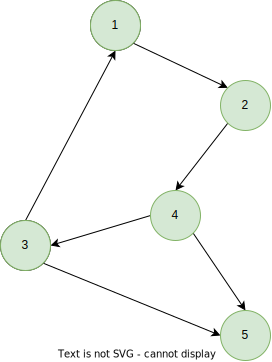
\includegraphics[width=0.35\textwidth]{diagrams/digraph0.drawio.png}
\end{center}

\begin{questions}
\question Implement the following graph operations using an adjacency matrix:

\begin{parts}
    \part Initialise a graph with n nodes.\lvlez
    \part Insert an edge in the graph \lvlez
    \part Delete an edge from the graph \lvlez
    \part Print the graph \lvlmed
    \part Deallocate the graph (free the memory for the nodes and the adjacency matrix) \lvlez
    \part Depth first search \lvlmed
    \part Breadth first search \lvlmed
\end{parts}

\question Implement the following graph operations using an edge list:

\begin{parts}
    \part Initialise a graph with n nodes.\lvlez
    \part Insert an edge in the graph \lvlmed
    \part Delete an edge from the graph \lvlmed
    \part Print the graph \lvlmed
    \part Deallocate the graph (free the memory for the nodes and the edge list) \lvlmed
    \part Depth first search \lvlmed
    \part Breadth first search \lvlmed
\end{parts}

\newpage
\question Implement the following graph operations using a data strucure similar to the following example:

\begin{lstlisting}[language=C]

typedef struct _NEIGHBOR_NODE{
    int key;
    struct _NEIGHBOR_NODE* next;
}NEIGHBOR_NODE;

typedef struct _GRAPH_NODE{
    int key;
    NEIGHBOR_NODE* first_neighbor;
    struct _GRAPH_NODE* next;
} GRAPH_NODE;

typedef struct{
    GRAPH_NODE* first_node;    
}GRAPH;
\end{lstlisting}


\includegraphics[width=\textwidth]{diagrams/digraph1.drawio.png}

Create a function for each of the following operations:
\begin{parts}
    \part Initialise the graph \lvlez
    \part Insert a node in the graph \lvlmed
    \part Delete a node from the graph \lvlmed
    \part Print the graph \lvlmed
    \part Insert an edge in the graph \lvlmed
    \part Delete an edge from the graph \lvlmed
    \part Deallocate the graph (free the memory for the nodes and the graph) \lvlmed
    \part Depth first search \lvlhard
    \part Breadth first search \lvlhard
\end{parts}

\end{questions}

\bigskip
\textbf{Note:} Leave a comment with the text PB1, PB2.A.II, ... PB10 above every function that implements the respective lab task. (upper case text, no space between the text and the problem number)

\medskip
\printbibliography
\end{document}
